\documentclass[aspectratio=169]{beamer}

\usepackage[brazil]{babel}
\usepackage[utf8]{inputenc}
\usepackage[T1]{fontenc}
\usepackage{graphicx}
\usepackage{amsmath}
\usepackage{booktabs}
\usepackage{tikz}

\usetheme{Madrid}
\usecolortheme{default}
\setbeamertemplate{navigation symbols}{}
\setbeamertemplate{footline}[frame number]
\setbeamertemplate{bibliography item}[text]

\definecolor{ufmgblue}{RGB}{0,55,110}
\definecolor{accentred}{RGB}{210,30,30}
\definecolor{darkgray}{RGB}{55,55,55}

\setbeamercolor{structure}{fg=ufmgblue}
\setbeamercolor{title}{fg=white,bg=ufmgblue}
\setbeamercolor{frametitle}{fg=white,bg=ufmgblue}
\setbeamercolor{block title}{fg=white,bg=ufmgblue}
\setbeamercolor{block body}{bg=black!3}
\setbeamercolor{alerted text}{fg=accentred}

\graphicspath{{../docs/report/figures/}}

\title[Planejamento em \texorpdfstring{\(SE(3)\)}{SE(3)}]{Planejamento de Movimento para Corpo Rígido em \texorpdfstring{\(SE(3)\)}{SE(3)}}
\subtitle{Geometria de \texorpdfstring{\(SE(3)\)}{SE(3)}, métrica logarítmica e interpolação}
\author{Pedro Antonio de Souza Campos Rodrigues}
\institute[UFMG]{Universidade Federal de Minas Gerais\\Programa de Pós-Graduação em Engenharia Elétrica}
\date{3 de julho de 2026}

\newcommand{\smalltag}[1]{\textcolor{darkgray}{\scriptsize #1}}

\begin{document}

\begin{frame}
    \titlepage
    \vspace{-0.8cm}
    \begin{center}
        
\includegraphics[height=0.7cm]{Logo_UFMG.png}
        \hspace{1.2cm}
        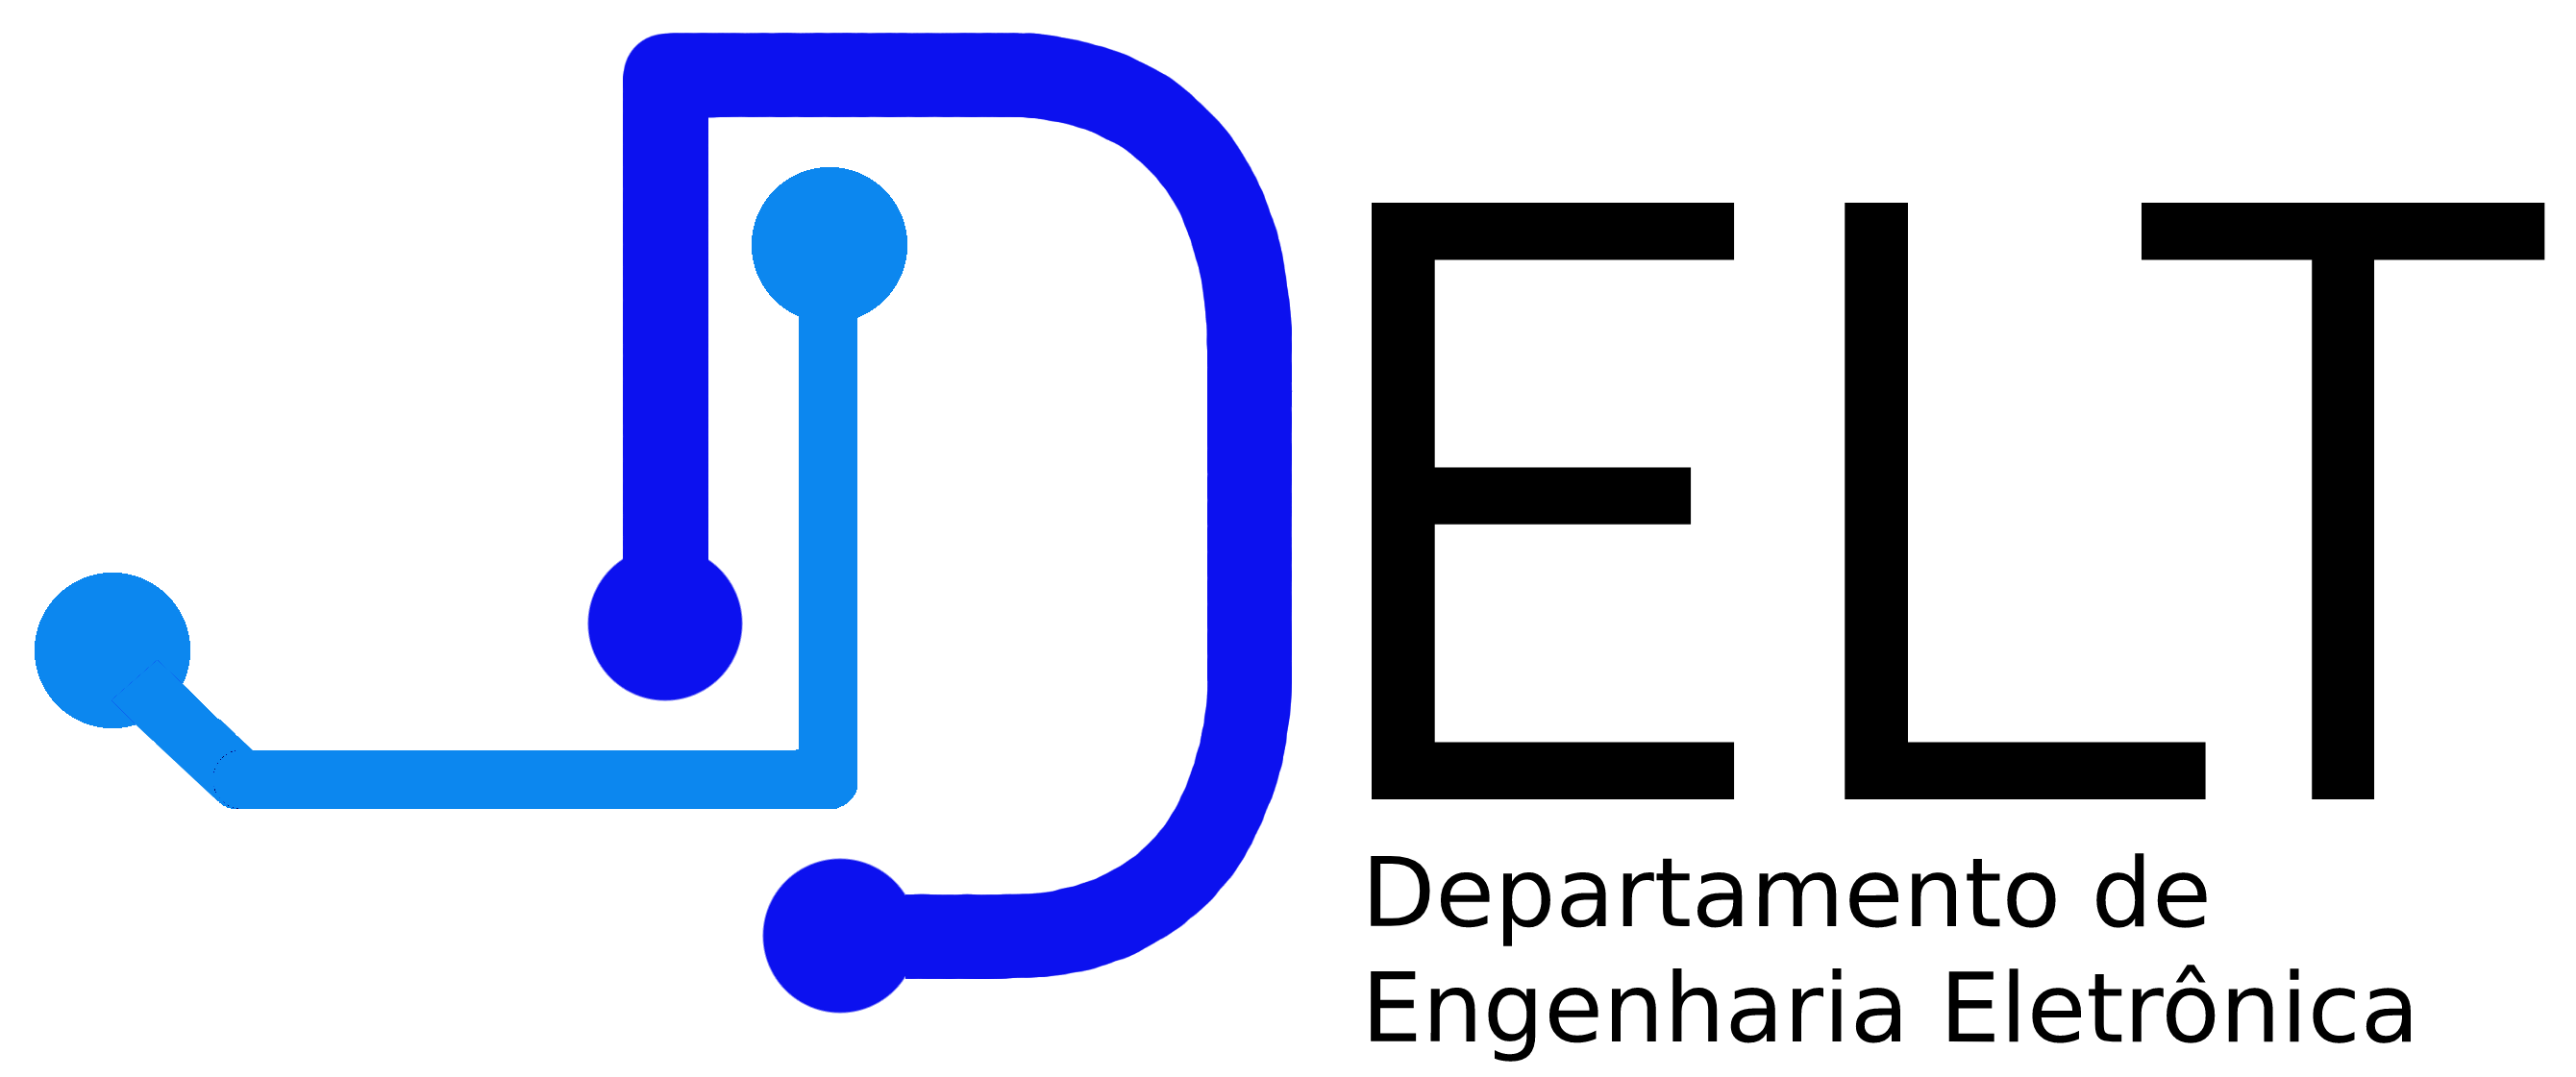
\includegraphics[height=0.7cm]{delt_logo.png}
    \end{center}
\end{frame}

\begin{frame}{Organização da Apresentação}
    \begin{enumerate}
        \item Representar a pose do corpo rígido.
        \item Definir uma distância entre duas poses.
        \item Interpolar e avançar entre poses em \(SE(3)\).
        \item Usar essas operações no RRT bidirecional.
        \item Apresentar o caminho retornado, o controle e os resultados.
    \end{enumerate}

    \vspace{0.35cm}
    \begin{block}{Ideia central}
        O ponto principal não é o RRT em si, mas como as poses são medidas e
        conectadas quando posição e orientação aparecem juntas.
    \end{block}
\end{frame}

\begin{frame}{Problema e Configuração}
    \begin{columns}[T]
        \begin{column}{0.46\textwidth}
            \textbf{Objetivo}
            \begin{itemize}
                \item sair de \(H_{\mathrm{start}}\);
                \item chegar em \(H_{\mathrm{goal}}\);
                \item planejar posição e orientação.
            \end{itemize}

            \vspace{0.2cm}
            \[
            H =
            \begin{bmatrix}
            R & p \\
            0 & 1
            \end{bmatrix}
            \in SE(3)
            \]
        \end{column}
        \begin{column}{0.50\textwidth}
            \textbf{Interpretação}
            \begin{itemize}
                \item \(R \in SO(3)\): orientação do corpo;
                \item \(p \in \mathbb{R}^3\): posição do corpo;
                \item cada ponto do caminho é uma pose completa;
                \item o planejador precisa medir, interpolar e avançar entre poses.
            \end{itemize}
        \end{column}
    \end{columns}

    \vspace{0.35cm}
    \smalltag{A representação por matrizes homogêneas é padrão em robótica para movimentos rígidos \cite{Murray1994,LynchPark2017}.}
\end{frame}

\begin{frame}{Erro entre Duas Poses}
    \small
    Para comparar \(H_1\) e \(H_2\), primeiro calcula-se a pose relativa:
    \[
    H_{\mathrm{rel}} = H_1^{-1}H_2.
    \]

    Em seguida, esse erro é escrito como um vetor de seis componentes:
    \[
    \xi =
    \vee\left(
    \log(H_1^{-1}H_2)
    \right),
    \qquad
    \xi =
    \begin{bmatrix}
    v \\
    \omega
    \end{bmatrix}.
    \]

    \begin{itemize}
        \item \(v\): parte translacional do erro;
        \item \(\omega\): parte angular do erro;
        \item a ordem adotada é sempre \([v;\omega]\).
    \end{itemize}

    \smalltag{O uso de exponencial e logaritmo para movimentos rígidos é apresentado, por exemplo, por Lynch e Park \cite{LynchPark2017}.}
\end{frame}

\begin{frame}{Distância Usada}
    \begin{block}{Métrica logarítmica ponderada}
        \[
        d(H_1,H_2)
        =
        \sqrt{\xi^\top G_\ell \xi},
        \qquad
        G_\ell =
        \mathrm{diag}(1,1,1,\ell^2,\ell^2,\ell^2)
        \]
    \end{block}

    \vspace{0.15cm}
    \begin{itemize}
        \item A distância é calculada a partir do erro relativo entre as poses.
        \item As três primeiras componentes medem deslocamento translacional.
        \item As três últimas componentes medem deslocamento angular.
        \item O parâmetro \(\ell\) define quanto uma rotação pesa em relação a uma translação.
    \end{itemize}

    \vspace{0.15cm}
    \begin{block}{Uso no planejamento}
        A mesma distância escolhe o nó mais próximo, limita o avanço, testa
        proximidade entre poses e define a discretização do caminho.
    \end{block}

    \vfill
    \smalltag{Park \cite{Park1995} discute a necessidade de ponderar translação e rotação ao definir distâncias entre movimentos rígidos.}
\end{frame}

\begin{frame}{Interpolação em \(SE(3)\)}
    \small
    Para conectar duas poses, primeiro calcula-se o deslocamento relativo de
    \(H_1\) até \(H_2\). A interpolação percorre uma fração desse deslocamento:

    \[
    H(s)
    =
    H_1
    \exp\left(
    s\log(H_1^{-1}H_2)
    \right),
    \qquad
    s\in[0,1].
    \]

    \vspace{0.1cm}
    \begin{itemize}
        \item \(H_1^{-1}H_2\) representa a pose de \(H_2\) vista a partir de \(H_1\).
        \item O logaritmo converte esse deslocamento em um incremento de pose.
        \item O fator \(s\) escolhe quanto desse incremento será aplicado.
        \item A exponencial transforma o incremento escalado novamente em uma pose.
    \end{itemize}

    \vspace{0.15cm}
    \begin{block}{Mensagem principal}
        O parâmetro \(s\) tem uma interpretação direta: \(s=0\) retorna \(H_1\),
        \(s=1\) retorna \(H_2\), e valores intermediários geram poses entre elas.
    \end{block}
\end{frame}

\begin{frame}{Por que Essa Interpolação?}
    \begin{itemize}
        \item Não interpolamos os elementos da matriz homogênea separadamente.
        \item A orientação permanece uma matriz de rotação válida.
        \item Posição e orientação evoluem juntas, como uma única pose.
        \item A mesma regra é usada no steering e na discretização do caminho.
    \end{itemize}

    \vspace{0.25cm}
    \begin{block}{Ideia principal}
        Cada aresta do RRT é uma conexão contínua entre poses, não apenas uma
        ligação reta entre posições.
    \end{block}
\end{frame}

\begin{frame}{Steering}
    \begin{block}{Avanço limitado}
        \[
        H_{\mathrm{new}}
        =
        H_{\mathrm{near}}
        \exp\left(
        \alpha
        \log(H_{\mathrm{near}}^{-1}H_{\mathrm{target}})
        \right)
        \]
    \end{block}

    \[
    \alpha =
    \min\left(
    1,
    \frac{\eta}{d(H_{\mathrm{near}},H_{\mathrm{target}})}
    \right).
    \]

    \begin{itemize}
        \item Se a pose alvo está perto, o avanço chega nela.
        \item Se está longe, o avanço percorre apenas uma fração do deslocamento.
        \item Assim, o steering é uma interpolação truncada pelo passo \(\eta\).
    \end{itemize}
\end{frame}

\begin{frame}{Amostragem de Poses}
    \footnotesize
    Cada amostra combina uma posição sorteada na caixa do cenário com uma
    orientação gerada por quaternion unitário.

    \[
    p =
    \begin{bmatrix}
    x & y & z
    \end{bmatrix}^{\top},
    \qquad
    q =
    \begin{bmatrix}
    q_0 & q_1 & q_2 & q_3
    \end{bmatrix}^{\top}.
    \]

    \begin{itemize}
        \item A posição é amostrada uniformemente dentro dos limites da caixa.
        \item Para a orientação, é gerado um vetor aleatório com quatro componentes seguindo uma distribuição normal padrão. Em seguida, esse vetor é normalizado para formar um quatérnio unitário.        \item Normaliza-se \(\bar{q}=q/\|q\|\), obtendo um quaternion unitário.
        \item O quaternion \(\bar{q}\) é convertido em uma matriz de rotação \(R\).
        \item Como \(\bar{q}\) é uniforme em \(S^3\), a rotação induzida é uniforme em \(SO(3)\).
    \end{itemize}

    \vspace{0.1cm}
    \begin{block}{Pose amostrada}
        A posição \(p\) e a rotação \(R\) formam a matriz homogênea \(H\).
        A orientação é gerada sem ângulos de Euler.
    \end{block}

    \smalltag{Quaternions unitários são usados classicamente para gerar rotações uniformes \cite{Shoemake1992}; a amostragem em planejadores é discutida por LaValle \cite{LaValle2006}.}
\end{frame}

\begin{frame}{RRT Bidirecional}
    \begin{block}{Como as operações anteriores aparecem no RRT}
        O RRT fornece a estrutura de exploração. A parte específica de \(SE(3)\)
        aparece nas operações realizadas a cada expansão.
    \end{block}

    \vspace{0.2cm}
    \begin{itemize}
        \item Amostragem: posição em uma caixa e orientação em \(SO(3)\).
        \item Nó mais próximo: definido pela métrica \(d(H_1,H_2)\).
        \item Expansão: feita pelo steering em \(SE(3)\).
        \item Conexão entre poses: gerada pela interpolação \(H(s)\).
    \end{itemize}

    \vfill
    \smalltag{RRTs e árvores bidirecionais são ferramentas clássicas de planejamento por amostragem \cite{LaValle2006,Choset2005,KuffnerLaValle2000}.}
\end{frame}

\begin{frame}{Caminho Retornado}
    \small
    O resultado do planejador é uma sequência de poses entre a configuração
    inicial e a configuração final:

    \[
    \mathcal{P}
    =
    \left\{
    H_0,\,
    H_1,\,
    \ldots,\,
    H_N
    \right\}.
    \]

    \begin{itemize}
        \item O caminho por waypoints representa a solução de forma compacta.
        \item O caminho discretizado é gerado interpolando poses consecutivas.
        \item A resolução \(\Delta_{\mathrm{out}}\) define a densidade do caminho final.
        \item Essa sequência discretizada é usada como referência para a etapa de seguimento.
    \end{itemize}

    \vspace{0.2cm}
    \begin{block}{Ponto importante}
        A saída final continua sendo um caminho em \(SE(3)\): cada ponto contém
        posição e orientação do corpo rígido.
    \end{block}
\end{frame}

\begin{frame}{Controle: Campo Vetorial e Modulação}
    \footnotesize
    Depois do planejamento, o caminho discretizado é usado como referência de
    seguimento. O controle adotado usa um campo vetorial em \(SE(3)\), na linha
    dos campos vetoriais construtivos discutidos por Bartelt et al. \cite{Bartelt2026}.

    \[
    \xi_d =
    \begin{bmatrix}
    v_d \\
    \omega_d
    \end{bmatrix},
    \qquad
    \xi = \alpha(d)\xi_d.
    \]

    \[
    d =
    \left\|
    \log\left(
    H^{-1}H_{\mathrm{goal}}
    \right)
    \right\|,
    \qquad
    \alpha(d)
    =
    1
    -
    e^{-\lambda d}
    \left(
    1+\lambda d
    \right).
    \]

    \begin{itemize}
        \item \(\xi_d\) combina avanço ao longo do caminho e correção em direção à referência.
        \item A modulação \(\alpha(d)\) reduz o twist quando o corpo se aproxima do alvo.
        \item Longe do alvo, \(\alpha(d)\approx 1\); perto do alvo, \(\alpha(d)\to 0\).
    \end{itemize}
\end{frame}

\begin{frame}{Resultados Preliminares}
    \begin{block}{Benchmark}
        Foram realizadas 100 execuções independentes no mesmo cenário, sem fixar
        semente aleatória.
    \end{block}

    \vspace{0.1cm}
    \begin{center}
        \begin{tabular}{lc}
            \toprule
            Métrica & Valor \\
            \midrule
            Execuções & 100 \\
            Sucessos & 100 \\
            Falhas & 0 \\
            Taxa de sucesso & \(100{,}00\%\) \\
            Tempo médio & \(0{,}022736\,\mathrm{s}\) \\
            Desvio padrão & \(0{,}010538\,\mathrm{s}\) \\
            \bottomrule
        \end{tabular}
    \end{center}

    \vspace{0.15cm}
    \smalltag{A variação de tempo é esperada em métodos baseados em amostragem aleatória \cite{LaValle2006}.}
\end{frame}

\begin{frame}{Conclusões}
    \begin{itemize}
        \item O planejamento foi formulado diretamente em termos de poses \(H\in SE(3)\).
        \item A métrica logarítmica ponderada permitiu comparar posição e orientação.
        \item A interpolação em \(SE(3)\) foi o bloco central para conectar poses.
        \item O steering reutiliza essa mesma interpolação, com limitação de passo.
        \item O RRT bidirecional usa essas operações para gerar o caminho.
        \item O caminho discretizado serve como referência para a etapa de seguimento.
    \end{itemize}
\end{frame}

\begin{frame}[allowframebreaks]{Referências}
    \tiny
    \bibliographystyle{plain}
    \bibliography{../docs/report/references}
\end{frame}

\end{document}
